% COMP1818 coursework report in the module's LaTeX template (COMPXXXX class, adapted from ECAI).
% Compile: pdflatex, bibtex, pdflatex, pdflatex (Overleaf: upload this whole folder).
% Rename this file to surname_firstname_AI_Intro.tex (your names) before submitting, if required.
% Every number comes from ../outputs (check with: python report/make_report_numbers.py).
\documentclass{COMPXXXX}
\usepackage{times}
\usepackage{graphicx}
\usepackage{latexsym}
\usepackage{amssymb}
\usepackage{amsmath}
\usepackage{booktabs}
\usepackage{multirow}
\usepackage{xcolor}
\usepackage{hyperref}

\newcommand{\pp}{\,pp}
\newcommand{\sx}{$\times$}

\begin{document}

\title{Investigating Deep Learning Techniques for Image Classification:\\
	Accuracy and Training Cost of EfficientNetV2 on Limited Data and Hardware}

\author{\textcolor{red}{[Firstname Surname]}\institute{School of Computing and Mathematical Sciences,
	University of Greenwich, London SE10 9LS, UK, email: \textcolor{red}{[your university email]},
	student ID: \textcolor{red}{[Student ID]}. COMP1818 Artificial Intelligence Applications.}}

\maketitle
\bibliographystyle{COMPXXXX}

\begin{abstract}
This study investigates whether the progressive learning of
EfficientNetV2~\cite{tan2021efficientnetv2}, which trains on small images with weak regularisation
before moving to larger images with stronger regularisation, still saves training time without losing
accuracy when a pretrained model is fine-tuned on a small image dataset. Four EfficientNetV2-S variants
(fixed 224\,px, growing image size only, the paper's full method, and the full method with Mixup) and
three baselines were trained for 12 epochs on the same 5{,}000 CIFAR-10 training images and 1{,}000
validation images, using a 4\,GB laptop GPU. On a separate test set of 2{,}000 images, the
fixed-resolution model achieved 95.35\% accuracy and a macro F1 score of 0.953, while the progressive
model achieved 95.50\% and 0.955 and needed 29\% less time for the same 12 epochs (1.40\sx, below the 1.56\sx\
predicted from FLOPs). Both were significantly more accurate than ResNet-18 (91.85\%) and far exceeded
HOG features with an SVM (54.10\%), although EfficientNetV2-S was 1.8 times larger than ResNet-18 and
2.5--2.7 times slower per image on a CPU. However, the differences among the four EfficientNetV2-S variants
were not statistically significant, and only one random seed was used, so progressive learning cannot
be said to improve accuracy.
\end{abstract}

% REQUIRED by the brief: a clearly labelled, accessible link to the implementation and dataset.
% Replace the red text, then test both links in a private/incognito browser window.
\noindent\fbox{\parbox{\dimexpr\columnwidth-2\fboxsep-2\fboxrule}{\small
\textbf{Implementation (code, trained models, logs):} \textcolor{red}{[paste OneDrive/Google Drive link]}\\
\textbf{Dataset:} CIFAR-10, \url{https://www.cs.toronto.edu/~kriz/cifar.html}; the exact
subset indices are in \texttt{outputs/splits.json} at the implementation link.}}

\section{Introduction}
Image classification assigns a category label to a photograph. It underpins applications such as
screening medical images, identifying crop diseases from phone photos, inspecting manufactured parts for
defects and sorting wildlife camera-trap images. In these settings labelled images are often scarce, and
the trained model may have to run on a laptop, a phone or an embedded device. Modern systems therefore
rarely learn from scratch: they fine-tune a network pretrained on ImageNet. Three questions then decide
which technique to use: how accurately it classifies, how much it costs to train, and how large and
fast it is once deployed.

EfficientNetV2~\cite{tan2021efficientnetv2} addresses the first two. Besides a fast-training
architecture, it introduces \emph{progressive learning}: images start small and grow during training,
and regularisation grows with them. The paper demonstrates this mainly for ImageNet-scale training; its
CIFAR-10 transfer experiment uses all 50{,}000 training images and 10{,}000 fine-tuning steps on large
accelerators. Whether the method still helps with a few thousand images, a short schedule and a laptop
GPU is unclear.

This study classifies CIFAR-10~\cite{krizhevsky2009learning} images with 500 training images per class.
It compares hand-crafted features (HOG\,+\,SVM), a standard CNN (ResNet-18) and four training variants
of EfficientNetV2-S under the same splits, preprocessing and optimiser, and asks:
\textbf{RQ1}: How much more accurate are pretrained deep networks than hand-crafted features, and
EfficientNetV2-S than ResNet-18?
\textbf{RQ2}: Is progressive learning as accurate as fixed-resolution fine-tuning, and which part of
it (growing the size, adapting regularisation, or this study's Mixup extension) matters?
\textbf{RQ3}: Does its FLOPs saving become a wall-clock saving on a laptop GPU, and what does each
model cost to deploy in size, speed and memory?

\section{Related Work}\label{sec:related}
The three model families compared here trace how image classification moved from human-designed
knowledge to learned representations. Dalal and Triggs's histograms of oriented
gradients~\cite{dalal2005histograms} describe an image by hand-chosen rules, counting local edge
directions in fixed cells, and pass these features to a support vector machine. The knowledge of
\emph{what} to look for is engineered explicitly, in the spirit of symbolic AI, while only the final
decision boundary is learned. Deep CNNs learn the features as well. ResNet~\cite{he2016deep} made very
deep networks trainable by adding residual (shortcut) connections, and pretrained ResNets became a
standard starting point for transfer learning. Efficient CNNs then reduced the cost of these networks
for limited hardware.

EfficientNetV2 builds on efficient CNNs that use MBConv blocks~\cite{sandler2018mobilenetv2} with
channel attention~\cite{hu2018squeeze}, architectures found by search~\cite{tan2019mnasnet,howard2019searching}
and compound scaling~\cite{tan2019efficientnet}. Because EfficientNet trained slowly, Tan and
Le~\cite{tan2021efficientnetv2} used \emph{Fused-MBConv}~\cite{gupta2020accelerator} in the early stages
and a search that also rewards training speed. Its \emph{progressive learning} splits training into $M$ stages; stage
$i$ uses image size $S_i$ and regularisation strengths $\phi_i^{k}$ (dropout,
RandAugment~\cite{cubuk2020randaugment} magnitude, Mixup~\cite{zhang2018mixup} $\alpha$), linearly
interpolated from start to end values:
\begin{equation}
S_i = S_0 + (S_e - S_0)\tfrac{i}{M-1},\qquad
\phi_i^{k} = \phi_0^{k} + (\phi_e^{k}-\phi_0^{k})\tfrac{i}{M-1}.
\label{eq:prog}
\end{equation}
The authors argue that small images carry less information and so need weaker regularisation, and
they attribute the accuracy drop of earlier progressive resizing to unchanged regularisation; B0
below tests this directly. For V2-S they use 128$\to$300\,px, RandAugment
5$\to$15, dropout 0.1$\to$0.3 and no Mixup, which they reserve for larger models.

Touvron et al.~\cite{touvron2019fixing} show that, because random crops make objects look larger
during training, testing at a moderately higher resolution than training improves accuracy, while a
large mismatch lowers it. We infer that this is one reason progressive training ends at its largest
size.

The closest prior result is the paper's own transfer experiment~\cite[Table~8]{tan2021efficientnetv2}:
EfficientNetV2-S, pretrained on ImageNet and fine-tuned on CIFAR-10, reached
$98.7\pm0.04$\% top-1 accuracy, averaged over five runs. That setting differs from this study's in four ways.
It used all 50{,}000 training images rather than 5{,}000. It fine-tuned for 10{,}000 steps at batch
size 512, about 100 passes over the data, rather than 12 epochs at batch size 32. It reports the mean
of five runs rather than a single run. Its image size is not stated in the transfer section, whereas
this study's is capped at 224\,px by a 4\,GB GPU. The 95.35--95.50\% reached here therefore measures how much of that
accuracy survives with a tenth of the data and a far smaller budget, not a like-for-like
reproduction.

\section{Experiment and Results}
\subsection{Setup}
\subsubsection{Dataset}
CIFAR-10~\cite{krizhevsky2009learning} contains 60{,}000 colour images of $32{\times}32$ pixels in ten
classes. Stratified, non-overlapping subsets were drawn with seed 42: 500 images per class for training
and 100 per class for validation from the official training set, and 200 per class (2{,}000 images)
for testing from the official test set. Images were upsampled to the training resolution and
normalised with ImageNet statistics; every deep model used random crops (4\,px padding) and horizontal
flips.

\subsubsection{Model Design and Training}
All deep models were ImageNet-pretrained torchvision~\cite{torchvision2016} checkpoints with a new
10-class head: EfficientNetV2-S (20.19\,M parameters) and ResNet-18~\cite{he2016deep} (11.18\,M). Each
was trained for 12 epochs with AdamW~\cite{loshchilov2019decoupled} (weight decay 0.05), one warm-up
epoch then cosine decay, batch size 32, label smoothing 0.1~\cite{szegedy2016rethinking} and mixed
precision. The learning rate $10^{-4}$ was chosen from $\{10^{-4}, 3{\times}10^{-4}, 10^{-3}\}$ by
validation accuracy in 3-epoch runs of variant A and used for every model. The four EfficientNetV2-S
variants were:
\begin{itemize}
\item \textbf{A} (fixed): 224\,px throughout, dropout 0.2, no RandAugment. ResNet-18 used the same settings.
\item \textbf{B0} (size only, first extension in this study): B's image sizes with A's regularisation, to separate
the effect of resizing (B0 vs A) from adapting regularisation (B vs B0).
\item \textbf{B} (paper recipe): size, RandAugment and dropout grow together over four 3-epoch stages
following Eq.~\eqref{eq:prog}, capped at 224\,px for the 4\,GB GPU (Table~\ref{tab:sched}).
\item \textbf{C} (Mixup ramp, second extension in this study): B plus Mixup, to test whether it helps V2-S when
only 5{,}000 images are available.
\end{itemize}

\begin{table}[t]
\centering\footnotesize
\caption{Progressive schedule for B and C. B0 uses only the size row.}
\label{tab:sched}
\begin{tabular}{@{}lcccc@{}}
\toprule
Stage (epochs) & 1 (1--3) & 2 (4--6) & 3 (7--9) & 4 (10--12) \\
\midrule
Image size (px) & 128 & 160 & 192 & 224 \\
RandAugment magnitude & 5 & 8 & 12 & 15 \\
Head dropout & 0.10 & 0.17 & 0.23 & 0.30 \\
Mixup $\alpha$ (C only) & 0 & 0.05 & 0.10 & 0.20 \\
\bottomrule
\end{tabular}
\end{table}

\subsubsection{Evaluation}
For each deep model, the epoch with the highest validation accuracy (always measured at 224\,px) was
selected and evaluated once on the 2{,}000 test images, which were used for no other choice. Accuracy is
the share of correctly classified images; macro-F1 averages the per-class F1 scores with equal weight;
mAP averages the one-vs-rest average precision of the ten classes. McNemar's
test~\cite{mcnemar1947note} checks whether two models differ, using the images that only one of them
classifies correctly. Baselines were uniform random guessing, always predicting the first class, and
HOG features~\cite{dalal2005histograms} with an RBF-kernel SVM ($C\in\{1,10\}$ chosen on validation).
Training cost is the wall-clock time of training steps only, on an NVIDIA RTX 2050 laptop GPU (4\,GB)
with PyTorch 2.14.1. Deployment cost was measured separately on the final models with random
$224{\times}224$ inputs, so no test image was reused: parameters, checkpoint size, FLOPs per image
(counted as twice the multiply-adds), latency for one image on the CPU (fp32), throughput for
batches of 32 on the GPU (fp16) and peak GPU memory. Timings are medians of repeated runs, and the
benchmark was run twice.

\subsection{Results}
\begin{table*}[t]
\centering\small
\caption{Test results on 2{,}000 CIFAR-10 images (one run per model, seed 42). Validation accuracy and
train--val gap are at the selected epoch; time is training-step wall-clock time; $p$ is McNemar's test
against A; mAP is one-vs-rest classification mAP (Section~3.1.3).}
\label{tab:main}
\resizebox{\textwidth}{!}{%
\begin{tabular}{@{}lccccccccc@{}}
\toprule
Model & Train res. (px) & Params (M) & Val acc. (\%) & Test acc. (\%) & Macro-F1 & mAP & Time (min) & Train--val gap (pp) & $p$ vs A \\
\midrule
Uniform random            & --          & --    & --    & 10.30 & 0.103 & --    & --    & --  & -- \\
Majority class            & --          & --    & --    & 10.00 & 0.018 & --    & --    & --  & -- \\
HOG + RBF-SVM ($C{=}1$)   & 32 (grey)   & --    & 54.30 & 54.10 & 0.541 & 0.542$^\ddagger$ & 0.1   & --  & $<10^{-100}$ \\
ResNet-18                 & 224         & 11.18 & 92.90 & 91.85 & 0.918 & 0.969 & 5.1   & 6.9 & $1.8{\times}10^{-8}$ \\
\midrule
A: EffNetV2-S, fixed      & 224         & 20.19 & 96.50 & 95.35 & 0.953 & 0.983 & 18.1  & 2.7 & -- \\
B0: progressive size only & 128$\to$224 & 20.19 & 96.10 & 95.05 & 0.951 & 0.977 & 12.4  & 3.1 & 0.58 \\
B: progressive (paper)    & 128$\to$224 & 20.19 & 96.70 & 95.50 & 0.955 & 0.987 & 12.9  & 0.1$^\S$ & 0.81 \\
C: B + Mixup ramp         & 128$\to$224 & 20.19 & 96.10 & 95.35 & 0.953 & 0.984 & 13.0  & n/a$^\dagger$ & 0.91 \\
\bottomrule
\end{tabular}}\\[1pt]
{\footnotesize $^\dagger$Not comparable under Mixup, where training accuracy uses mixed labels.
$^\S$Measured on harder RandAugment inputs; see text.
$^\ddagger$From one-vs-rest SVM decision margins, not probabilities.}
\end{table*}

\paragraph{Accuracy (RQ1, RQ2).} Table~\ref{tab:main} shows that both trivial baselines sit at chance,
confirming balanced splits. Pretrained deep networks far outperformed hand-crafted features: HOG + SVM
reached 54.10\%, every deep model over 91\%. With the same recipe, EfficientNetV2-S (A) was 3.5\pp\ more
accurate than ResNet-18 (95.35 vs 91.85\%, $p=1.8{\times}10^{-8}$), at 3.5\sx\ the training time; all four
variants beat ResNet-18 significantly ($p\leq3.2{\times}10^{-7}$). Among the variants, B scored highest
(95.50\%, macro-F1 0.955, mAP 0.987), but \emph{no pair among A, B0, B and C differed significantly}
(all $p>0.3$). The 95\% confidence interval on one accuracy is about $\pm0.9$\pp, larger than the
0.45\pp\ spread between the variants.

\begin{figure}[t]
\centering
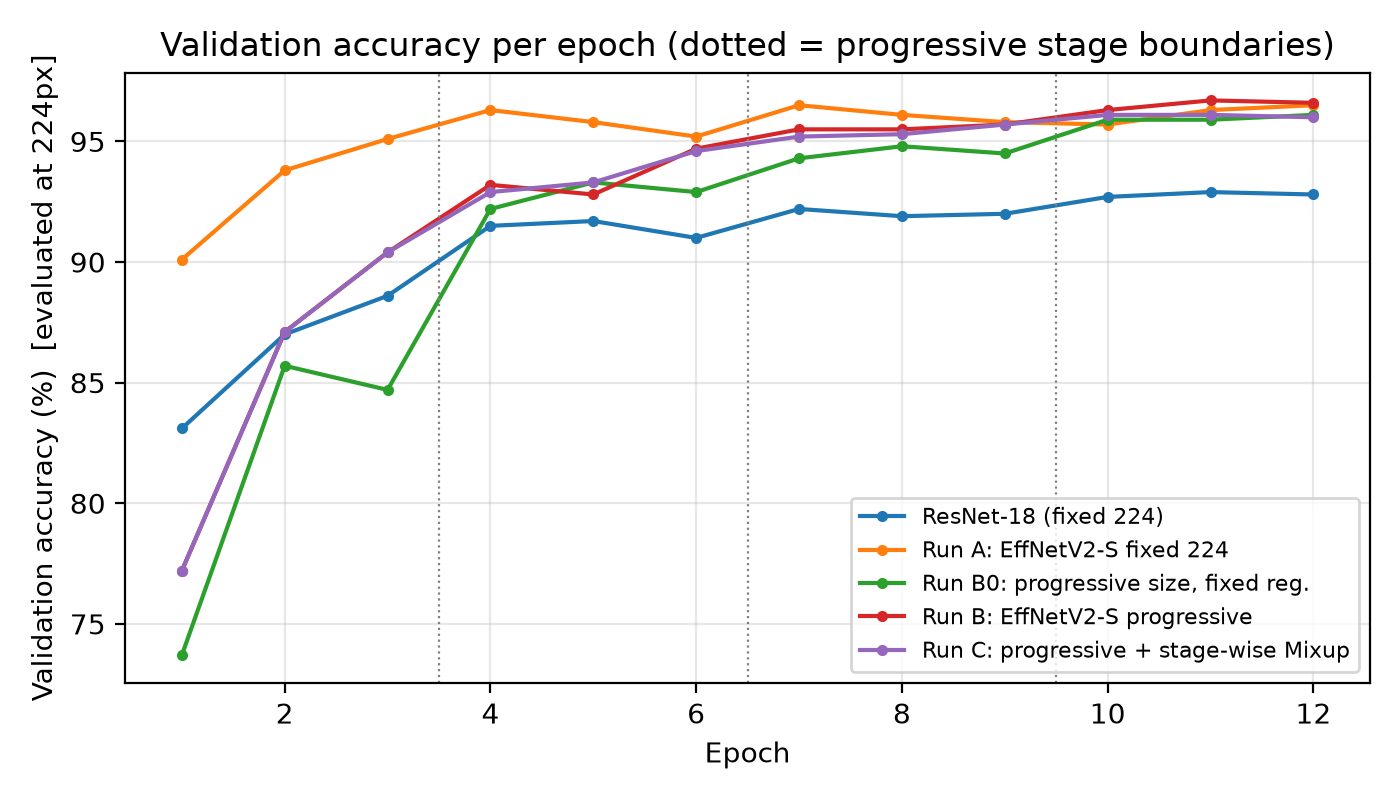
\includegraphics[width=\columnwidth]{figures/val_acc_comparison.png}
\caption{Validation accuracy (at 224\,px) per epoch. Dotted lines mark the stage boundaries of B0, B
and C.}
\label{fig:val}
\end{figure}

\paragraph{Learning curves.} In Figure~\ref{fig:val}, the progressive variants started 13--16\pp\ below
A because they trained at 128\,px but were validated at 224\,px~\cite{touvron2019fixing}; the gap had
closed by stage~4, when the resolutions matched. A and B0 reached about 99\% training accuracy (a
2.7--3.1\pp\ gap to validation), whereas B's gap was smaller (0.1\pp\ at the selected epoch, 0.6\pp\ at
epoch 12) at equal or higher validation accuracy. Part of this is how it was measured: B's training
accuracy comes from harder RandAugment images, so the smaller gap is not clear evidence of less overfitting.

\paragraph{Class-level performance.} Figure~\ref{fig:cm} shows predictions per class. Frog had the
highest recall under both A and B (197 of 200) and cat the lowest (174 and 179). For A, B and ResNet-18
the most common confusion, counting both directions, was between cat and dog (25 errors under A, 21
under B; a cat predicted as a dog 17 and 13 times), followed by automobile and truck in either direction
(12 and 13). B classified more cats, birds, automobiles and horses correctly
than A, but fewer trucks (189 vs 194), ships (193 vs 196) and dogs (185 vs 187), so its small lead is
not consistent across classes.

\begin{figure*}[t]
\centering
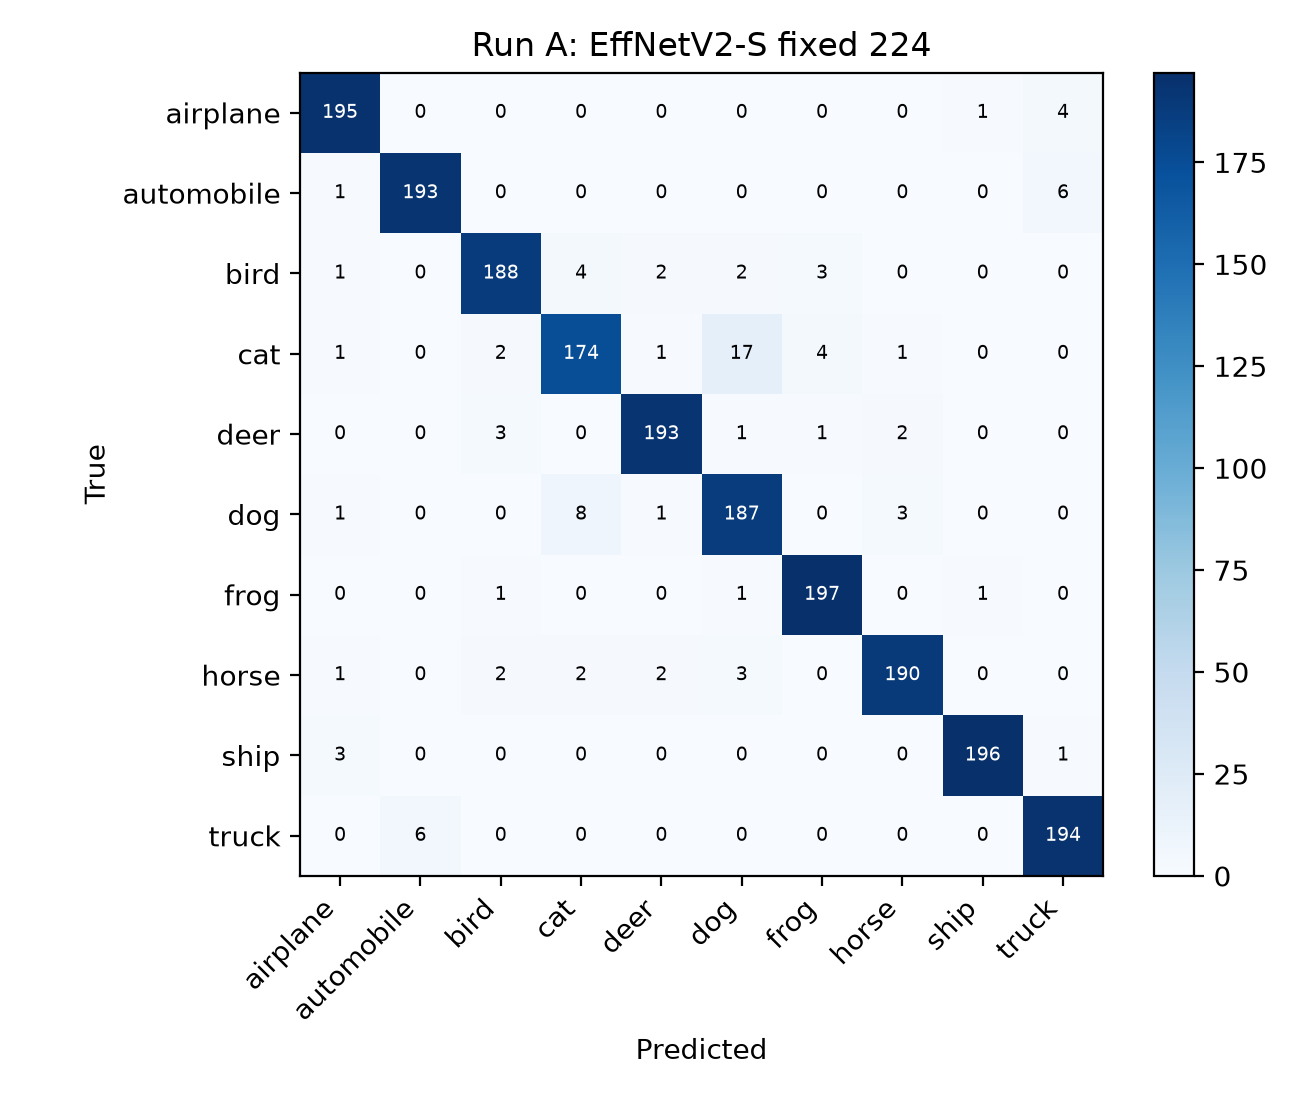
\includegraphics[width=0.36\textwidth]{figures/cm_A_effnetv2s_fixed224.png}\hspace{2em}
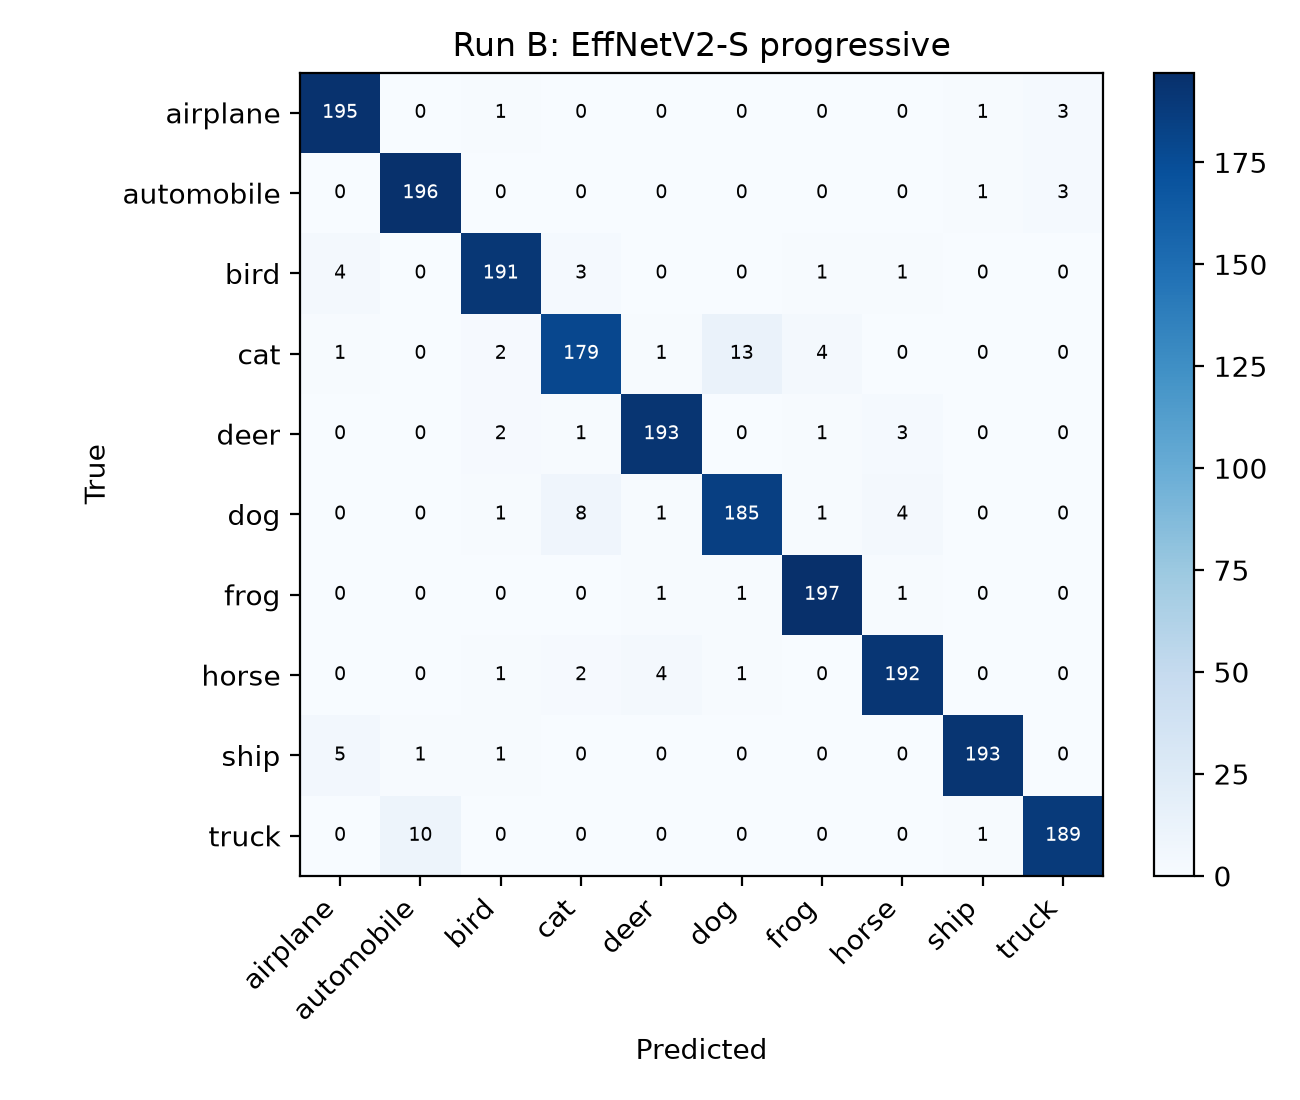
\includegraphics[width=0.36\textwidth]{figures/cm_B_effnetv2s_progressive.png}
\caption{Test confusion matrices for A (left) and B (right). Rows are true labels; columns are
predictions; each class has 200 test images.}
\label{fig:cm}
\end{figure*}

\paragraph{Training cost (RQ3).} For the same 12 epochs, training time fell from 18.1\,min (A) to
12.9\,min (B, 1.40\sx), 12.4\,min (B0, 1.45\sx) and 13.0\,min (C, 1.39\sx). This is a per-epoch saving, not
a shorter time to a given accuracy: A first reached 96.3\% validation accuracy at epoch~4 (5.9\,min), B
only at epoch~10 (9.9\,min). Differences of about 1\pp\ on 1{,}000 validation images are mostly noise, so
neither variant was clearly faster to reach a given accuracy.
FLOPs grow with $(S/224)^2$, predicting 0.643 of A's cost
(1.56\sx). A least-squares fit over all 48 EfficientNetV2-S epochs gives
\begin{equation}
t_{\text{epoch}}(S) \approx 15.7\,\text{s} + 74.8\,\text{s}\cdot(S/224)^2,\qquad R^2=0.991,
\label{eq:cost}
\end{equation}
which predicts a ratio of 0.705, within 0.02 of each measured value: about 17\% of a 224\,px epoch is a
fixed cost that does not shrink with image size. Peak GPU memory was unchanged (2.62--2.63\,GB), as it
is set by the final 224\,px stage.

\begin{table}[t]
\centering\footnotesize
\caption{Deployment cost of the final models (224\,px input; all EfficientNetV2-S variants share one
architecture). Ranges span two benchmark runs. CPU: one image, fp32. GPU: RTX~2050, fp16, batches of 32.}
\label{tab:deploy}
\setlength{\tabcolsep}{3pt}
\resizebox{\columnwidth}{!}{%
\begin{tabular}{@{}lcccccc@{}}
\toprule
Model & Params (M) & Size (MB) & GFLOPs & CPU ms/image & GPU images/s & GPU mem (GB) \\
\midrule
HOG + SVM       & --$^\ast$ & 13.1 & --   & 1.3--1.4 & --         & --   \\
ResNet-18       & 11.18     & 44.8 & 3.63 & 19--21   & 1{,}050--1{,}060 & 0.42 \\
EffNetV2-S      & 20.19     & 81.6 & 5.70 & 50--51   & 338--340   & 0.30 \\
\bottomrule
\end{tabular}}\\[1pt]
{\footnotesize $^\ast$The SVM stores 4{,}794 support vectors of 324 HOG features.}
\end{table}

\paragraph{Deployment cost (RQ3).} Table~\ref{tab:deploy} shows the price of EfficientNetV2-S's
3.5\pp\ accuracy gain over ResNet-18 at inference. It has 1.8\sx\ the parameters and checkpoint size and
1.6\sx\ the FLOPs, yet it was 2.5--2.7\sx\ slower per image on the CPU and processed 3.1\sx\ fewer images per
second on the GPU. On the GPU with single images it took 24--36\,ms against 3.7--3.8\,ms for ResNet-18,
a latency that varied between runs. HOG + SVM was the smallest and fastest, at 1.3--1.4\,ms per image
on the CPU, but its accuracy (54.10\%) rules it out.

\section{Discussion}
For classification accuracy (RQ1), pretrained deep features matter most: the 38--41\pp\ gap between
HOG + SVM and the deep models dwarfs every other difference. That gap combines two factors, learned
versus hand-chosen features and ImageNet pretraining, which this study cannot separate because no deep
model was trained from scratch. Architecture comes next: EfficientNetV2-S was
significantly more accurate than ResNet-18 under an identical recipe, though it has more parameters and
trained 3.5\sx\ longer, so the gain cannot be attributed to its design alone.

For RQ2, there is no evidence that progressive learning costs accuracy, but the experiment cannot show
that the variants are equivalent: with one seed and 2{,}000 test images, differences below about 1\pp\
are not resolvable. Resizing alone (B0 vs A) changed accuracy by $-0.30$\pp\ ($p=0.58$), adaptive
regularisation (B vs B0) by $+0.45$\pp\ ($p=0.35$) with a smaller measured train--validation gap
(partly an effect of measuring on harder images), and the
Mixup ramp (C vs B) by $-0.15$\pp\ ($p=0.79$). None is significant. CIFAR-10 also limits this test:
every resolution is an interpolation of the same $32{\times}32$ image, so small stages lose no
information, which weakens the paper's argument that small images need less regularisation.

For RQ3, the cost model attributes the shortfall from 1.56\sx\ to a fixed cost per epoch. Likely
sources are the small GPU, the batch of 32 and single-process data loading, though these were not
profiled. FLOPs, as EfficientNetV2 itself argues~\cite{tan2021efficientnetv2}, do not equal training time,
and the deployment results show the same at inference: EfficientNetV2-S needs 1.6\sx\ ResNet-18's
FLOPs but runs 2.5--3.1\sx\ slower, plausibly because of its many depthwise convolutions, which the
same paper notes cannot fully use modern accelerators~\cite{tan2021efficientnetv2}, and its small
squeeze-and-excitation operations. For deployment, the choice therefore depends on the application:
EfficientNetV2-S where every percentage point of accuracy matters, ResNet-18 where latency or device
size dominates. Progressive learning changes only training, so it has no effect on these
inference costs. These measurements use unoptimised PyTorch on one laptop; quantisation or a dedicated
inference engine could change the ratios.

Other limitations: the learning rate was tuned on A and reused, which may slightly favour A; selecting
the best epoch on 1{,}000 validation images is mildly optimistic for every model; and compared with
the paper's CIFAR-10 transfer experiment (Section~\ref{sec:related}), the study used a tenth of the
training images, 12 epochs instead of about 100, one run instead of five, and images capped at
224\,px. Under these limits, B's 95.50\% is 3.2\pp\ below the paper's 98.7\%, about 97\% of its
accuracy at a fraction of its budget. The study therefore tests the
mechanism in a low-data transfer setting rather than reproducing the paper's reported numbers.

\section{Conclusion and future work}
This study compared techniques for classifying CIFAR-10 images with 500 training images per class on a
4\,GB laptop GPU. Pretrained deep networks far outperformed HOG + SVM (54.10\%), and EfficientNetV2-S was
significantly more accurate than ResNet-18 (95.35 vs 91.85\%, $p=1.8{\times}10^{-8}$), reaching about 97\%
of EfficientNetV2's reported 98.7\%~\cite{tan2021efficientnetv2} with a tenth of its data and about a
tenth of its epochs. Progressive learning was not significantly different from fixed-resolution
fine-tuning (95.50 vs 95.35\%, $p=0.81$) and cut training time for the same 12 epochs by 29\%, less
than the 36\% implied by FLOPs, consistent with a fixed per-epoch cost; it did not improve accuracy
and was not shown to reach a given accuracy sooner. Neither adaptive regularisation nor Mixup changed
accuracy significantly. At inference, EfficientNetV2-S's accuracy gain over ResNet-18 costs 1.8\sx\
the model size and 2.5--2.7\sx\ the CPU latency.
\textcolor{red}{[Your one-sentence practical takeaway: which technique to use, and when.]}
Future work could use several random seeds, natively high-resolution images where small stages
genuinely remove detail, a deep model trained from scratch to separate pretraining from learned
features, a learning rate tuned for each variant, time to a target accuracy rather than a fixed
number of epochs, and faster data loading to recover more of the FLOPs saving.

% REQUIRED by the brief: 60-100 words, written by you, placed after the report and BEFORE the
% references. Cover: (1) AI tool(s) used; (2) how AI supported your learning; (3) how AI outputs
% were edited, transformed or expanded; (4) how outputs were verified and errors corrected.
% Be specific and honest about what AI produced (code, figures, text) and what you did yourself.
\section*{Reflection on the use of AI}
\textcolor{red}{[Write your 60--100 word reflection here.]}

\bibliography{references}

\end{document}
